% coding:utf-8

%FOSAET, a LaTeX-Code for a electrical summary of basic electronics
%Copyright (C) 2013, Daniel Winz, Ervin Mazlagic

%This program is free software; you can redistribute it and/or
%modify it under the terms of the GNU General Public License
%as published by the Free Software Foundation; either version 2
%of the License, or (at your option) any later version.

%This program is distributed in the hope that it will be useful,
%but WITHOUT ANY WARRANTY; without even the implied warranty of
%MERCHANTABILITY or FITNESS FOR A PARTICULAR PURPOSE.  See the
%GNU General Public License for more details.
%----------------------------------------

\newpage
\section{Stromteiler}
\begin{figure}[h!]
	\centering
	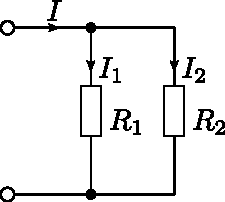
\includegraphics[scale=\schscale]{iteil.pdf}
	\caption{Stromteiler}
	\label{sch:iteil}
\end{figure}
\[ I_2 = I \cdot \frac{R_1}{R_1 + R_2} \]

\subsubsection{Stromteiler mit $> 2$ Widerständen}
\[ I_n = I_q \cdot \frac{(R1 // R2 \dots // R_{n-1})}
{(R1 // R2 \dots // R_{n-1}) + R_n} 
= I_q \cdot \frac{\left(\frac{R_1 \cdot R_2 \dots R_{n-1}}
{R_1 + R_2 \dots R_{n-1}}\right)}
{\left(\frac{R_1 \cdot R_2 \dots R_{n-1}}
{R_1 + R_2 \dots R_{n-1}}\right) + R_n} \]